\section{The Household Population}
\label{ch:population}

We construct a synthetic population of 5{,}000 household agents from South African microdata.
This section outlines the data sources, variable derivations, financial indicator imputations, and empirical validation of the static population structure.
Dynamic household interactions and behavioural realism are evaluated separately in Section~\ref{sec:results-baseline}.
All monetary figures are denominated in 2017 South African Rand (ZAR) matching the base survey year, with no inflation adjustments applied at the data layer.

\subsection{Primary Dataset: NIDS Wave 5}
\label{sec:backbone}

The backbone of the synthetic population is drawn from \ac{NIDS} Wave 5 \cite{nids_w5_2018}.
Filtering the raw sample ($N = 13,719$) for households with reported income, valid size, and
positive sampling weights leaves 10{,}841 records. The 2{,}878 discarded records carry zero or missing weights; their removal thus entails no loss of weighted population mass. Scaled by national design weights, the final sample represents 18.67 million households or roughly 56.5 million individuals.

We derive six core economic variables per household: monthly income and its dominant source (wage, grant, or remittance and other); committed expenditure (food and rent paid, an incompressible floor); discretionary expenditure (all other non-food cash spending); liquid savings (financial assets, winsorised at the 99th percentile); and traditional debt (outstanding financial debt).
Imputed rent, the non-cash consumption value of owner-occupied housing, is excluded from both expenditure tiers.
Appendix~\ref{app:variables} gives the source field, formula, missing-data treatment and diagnostics for every variable, including the debt-service construction of Section~\ref{sec:servicing}.

Four survey fields record values only when an asset or liability is present, so a missing entry denotes non-holding and is set to zero: financial assets (unobserved for 48.2\% of households), financial debt (56.6\%), total debt (54.4\%), and rent paid (80.2\%).
Section~\ref{sec:data-validation} tests this assumption against aggregate national credit data; operationally it means that committed expenditure reduces to food costs alone for home-owning households.

Households are stratified into per-capita income quintiles bounded at ZAR 900, ZAR 1{,}801, ZAR 3{,}400, and ZAR 7{,}712 per month.
Demographic variables for the household head (age, gender, race, education) are merged from the \ac{NIDS} individual file, matching 10{,}736 of the 10{,}841 retained households.

\subsection{Imputing Financial Inclusion: FinScope 2019}
\label{sec:match}

Because \ac{NIDS} omits institutional banking status and specific debt instruments, we impute six binary financial inclusion indicators from the 2019 \ac{FinScope} survey \cite{finscope2019}.
Banked status determines entry into \ac{BNPL}, bounding potential market adoption at the observed 82.8\% macro limit rather than an arbitrary baseline parameter.
Five credit-product flags (store cards, revolving credit, hire purchase, short-term loans, and personal loans) determine the interest rates and repayment schedules assigned in Section~\ref{sec:servicing}.
Unused indicator fields are omitted.

We transfer attributes using cell-donor matching, illustrated in Figure~\ref{fig:cell-donor}.
Stratifying both datasets by per-capita income quintile and province, each \ac{NIDS} record draws a donor from its matching cell with probability proportional to the donor's survey weight (seed: 42).
Extracting all six indicators from a single donor preserves the joint product distribution.
Each of the 45 sampling cells contains at least 30 donor candidates, and no draw ever fell back to a coarser cell.

Three properties of the match matter for what follows.
Because one donor supplies all six flags, the imputed joint distribution of products is a real household's rather than a product of six independent marginals, which matters because stacking is a joint phenomenon.
Because nothing within a cell is matched on, the imputation reproduces between-cell variation in inclusion and suppresses within-cell variation, so the eligible population is more homogeneous than the real one.
And because the flags are two years younger than the population, the 82.8\% banked ceiling is plausibly slightly generous for 2017.
Appendix~\ref{app:matching} states the assumptions under which the match is credible, the circumstances under which it is not, and which of them would move a headline result.

\begin{figure}[H]
\centering
\begin{tikzpicture}[font=\footnotesize, >=Stealth,
  cell/.style={draw, minimum width=0.46cm, minimum height=0.34cm, inner sep=0pt},
  hl/.style={fill=black!18},
  rec/.style={draw, rounded corners=1pt, align=center, inner sep=4pt},
  donor/.style={circle, draw, fill=black!8, inner sep=0pt},
  lbl/.style={align=center}]
% ---- panel (a): the same partition of both surveys --------------------------
\node[lbl] at (-0.55,2.2) {\textbf{(a)}};
\foreach \x in {0,...,8} \foreach \y in {0,...,4} {
  \node[cell] at (\x*0.46, \y*0.34) {};
  \node[cell] at (6.7+\x*0.46, \y*0.34) {};
}
\node[cell, hl] (rcell) at (2*0.46, 3*0.34) {};
\node[cell, hl] (dcell) at (6.7+2*0.46, 3*0.34) {};
\foreach \y/\l in {0/Q1,1/Q2,2/Q3,3/Q4,4/Q5} {
  \node[left, font=\scriptsize] at (-0.28,\y*0.34) {\l};
  \node[left, font=\scriptsize] at (6.42,\y*0.34) {\l}; }
\node[lbl] at (1.85,-0.68) {\textbf{NIDS 2017}, 10{,}841 recipients\\[-2pt] \scriptsize nine provinces $\rightarrow$};
\node[lbl] at (8.55,-0.68) {\textbf{FinScope 2019}, 4{,}969 donors\\[-2pt] \scriptsize nine provinces $\rightarrow$};
\draw[->, thick] (rcell.north) to[out=75, in=105] node[midway, above, lbl]
  {the same cell $c = (q, p)$: 45 cells, each with at least 30 donors} (dcell.north);
% ---- panel (b): one donor, the whole vector ---------------------------------
\node[lbl] at (-0.55,-1.7) {\textbf{(b)}};
\node[rec] (recip) at (1.5,-2.9) {recipient $i$\\[1pt] \scriptsize income, expenditure,\\[-1pt] \scriptsize savings, debt from \ac{NIDS}};
\node[donor, minimum size=14pt, fill=black!40] (d3) at (8.55,-2.9) {};
\node[donor, minimum size=6pt]  (d6) at (8.9,-2.2) {};
\node[donor, minimum size=5pt]  (d1) at (9.45,-2.4) {};
\node[donor, minimum size=9pt]  (d2) at (10.05,-2.75) {};
\node[donor, minimum size=7pt]  (d4) at (10.55,-3.2) {};
\node[donor, minimum size=11pt] (d5) at (9.4,-3.4) {};
\node[draw, dashed, fit=(d1)(d2)(d3)(d4)(d5)(d6), inner sep=5pt,
  label={[lbl, font=\scriptsize, yshift=-2pt]below:donor pool of cell $c$;\\ circle area $\propto$ weight $w_d$}] (pool) {};
\draw[->, thick] (d3.west) -- (recip.east)
  node[midway, above, lbl, yshift=1pt] {one donor $d$, drawn with\\ probability $w_d / \sum_{d' \in c} w_{d'}$}
  node[midway, below, lbl, font=\scriptsize, yshift=-1pt] {copies the whole\\ six-flag vector};
% ---- panel (c): the rejected alternative ------------------------------------
\node[lbl] at (-0.55,-4.75) {\textbf{(c)}};
\node[rec] (recip2) at (1.5,-5.7) {recipient $i$\\[1pt] \scriptsize per-flag imputation\\[-1pt] \scriptsize (rejected)};
\foreach \k/\ypos in {1/-4.95,2/-5.25,3/-5.55,4/-5.85,5/-6.15,6/-6.45} {
  \node[donor, minimum size=6pt] (e\k) at (8.55,\ypos) {};
  \draw[->, thin] (e\k.west) -- (recip2.east); }
\node[lbl, right, font=\scriptsize] at (8.85,-5.7) {six draws from six\\ different donors: the same\\ marginals, but the joint\\ structure stacking depends\\ on is lost};
\end{tikzpicture}
\caption{The cell-donor match}
\label{fig:cell-donor}
\tabnote{Panel (a): both surveys are partitioned into the same 45 cells by per-capita income quintile and province; a \ac{NIDS} household draws its donor only from the \ac{FinScope} households in its own cell, and every cell holds at least 30 donors. Panel (b): within the cell, one donor is drawn with probability proportional to its survey weight (circle area), and its entire six-flag vector is copied to the recipient, so the imputed joint distribution of products is a real household's. Panel (c): the rejected alternative, one draw per flag from six different donors, reproduces the same marginals but discards the joint structure that concurrent-facility stacking depends on. Appendix~\ref{app:matching} gives the procedure formally, with its assumptions and limits.}
\end{figure}

\ac{FinScope} reports income in seven discrete bands rather than continuously; we place donors into quintiles using band midpoints divided by household size.
Deflating 2019 income brackets to 2017 Rands shifts imputed quintile rates by at most 2.4 percentage points, so we retain the unadjusted key.

Table~\ref{tab:imputation_errors} shows national target matches, where the maximum absolute discrepancy is 1.8 percentage points (store cards).
Figure~\ref{fig:inclusion-fidelity} breaks down alignment across quintiles; the maximum deviation across all thirty quintile-by-indicator cells is 2.3 percentage points.

\begin{table}[H]
\centering
\caption{National rates for the six imputed indicators}
\label{tab:imputation_errors}
\tabnote{This table compares the national rate of each imputed indicator in three populations: the \ac{FinScope} 2019 benchmark, weighted by its survey weight; the 10{,}841-household synthetic population after matching, weighted by \ac{NIDS} survey weight; and the unweighted 5{,}000-agent resample used in the simulation. The difference column is synthetic less \ac{FinScope}, in percentage points, computed before rounding; the tolerance is 3 percentage points (Table~\ref{tab:validation}). Because the match draws donors within the same quintile-by-province cell in proportion to weight, agreement here is expected by construction: it tests the implementation, not the population's external validity (Appendix~\ref{app:matching}).}
\begin{tabular}{lrrrr}
\toprule
\textbf{Imputed indicator} & \textbf{FinScope 2019} & \textbf{Synthetic} & \textbf{Agents} & \textbf{Difference} \\
 & \textbf{(\%)} & \textbf{(\%)} & \textbf{(\%)} & \textbf{(pp)} \\
\midrule
Banked status    & 82.4 & 82.8 & 82.8 & 0.4 \\
Store card       & 20.8 & 22.6 & 21.8 & 1.8 \\
Revolving credit &  3.7 &  4.1 &  3.8 & 0.5 \\
Hire purchase    &  6.5 &  6.9 &  6.5 & 0.5 \\
Short-term loan  &  2.7 &  3.4 &  3.3 & 0.6 \\
Personal loan    &  2.1 &  2.3 &  2.3 & 0.2 \\
\bottomrule
\end{tabular}
\end{table}

\begin{figure}[htbp]
\centering
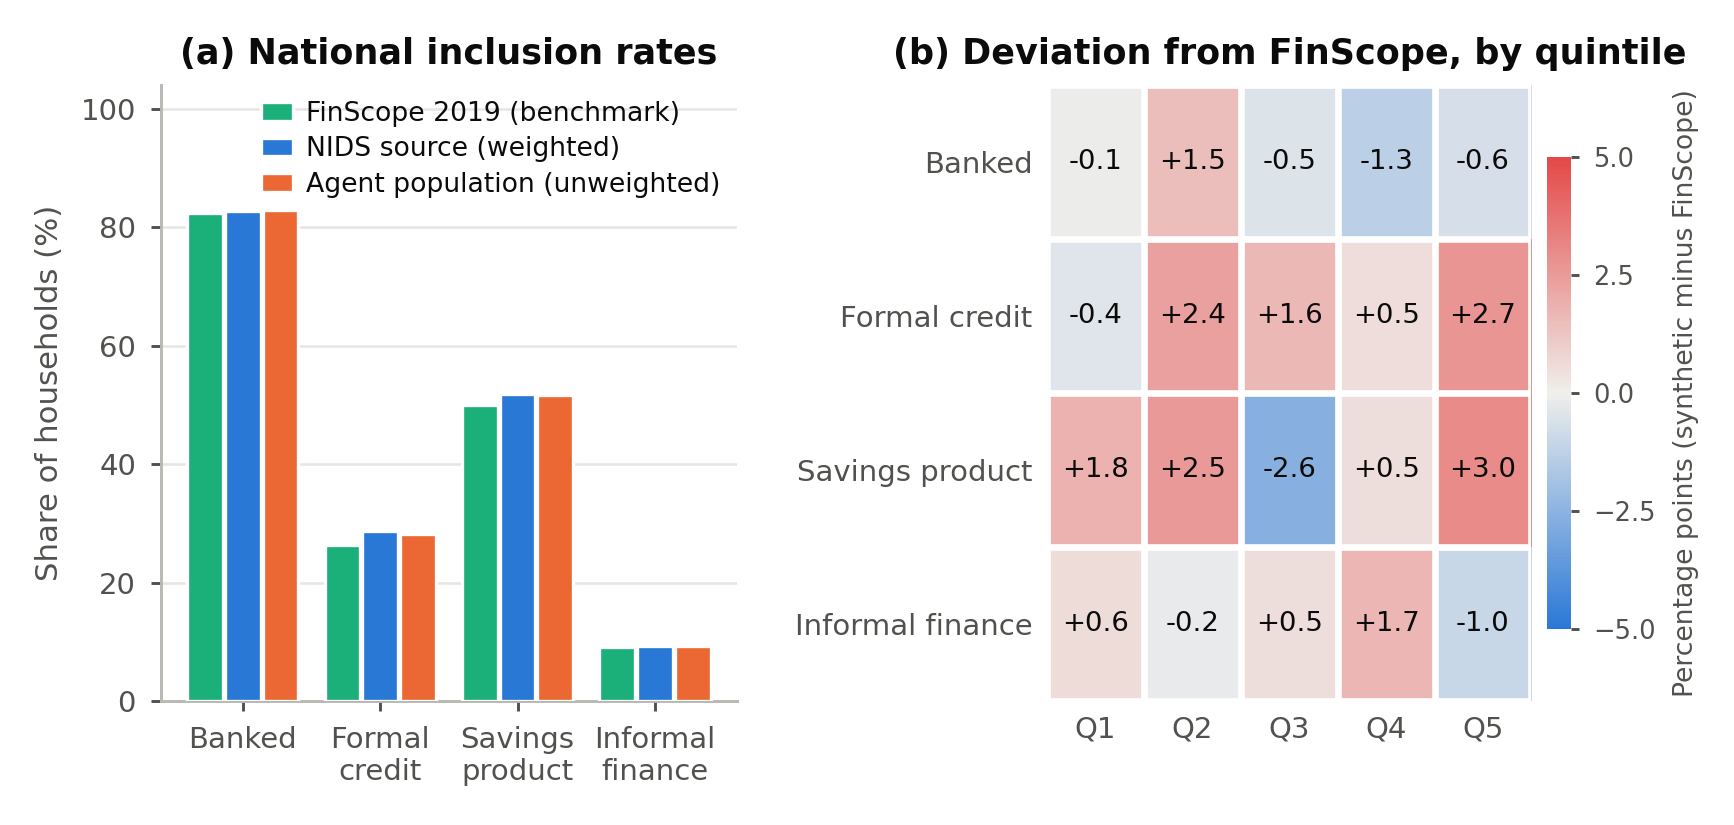
\includegraphics[width=\textwidth]{figures/fig_inclusion_fidelity.pdf}
\caption{Fidelity of the imputed indicators}
\label{fig:inclusion-fidelity}
\tabnote{Panel (a) compares the national rate of each of the six imputed indicators across the \ac{FinScope} 2019 benchmark, the weighted synthetic population and the unweighted 5{,}000-agent population, as in Table~\ref{tab:imputation_errors}. Panel (b) shows the synthetic-less-\ac{FinScope} gap for each indicator within each per-capita income quintile, thirty cells in all; the largest single deviation is 2.3 percentage points against a tolerance of 5. Quintiles are the weighted \ac{NIDS} bounds of Section~\ref{sec:backbone}.}
\end{figure}

The geographic and income-based cells establish the reporting categories for quintile-level analysis and define the reference networks that drive peer-influence dynamics in the simulation.

\subsection{Debt Servicing Construction}
\label{sec:servicing}

\ac{NIDS} measures debt \emph{stocks}, but the simulation requires monthly cash \emph{flows}.
Monthly debt service is reconstructed in three steps, specified in full in Appendix~\ref{app:variables}: each household's balance is amortised at the \ac{NCA} statutory maximum \ac{APR} for 2017 \cite{sa_ncr_ratecaps_2016} over a product-specific repayment horizon (Table~\ref{tab:credit-terms}), and the resulting instalment is capped at the Regulation 23A residual-income ceiling \cite{sa_ncr_affordability_2015}.
Because realised rates by product class are unobserved in the \ac{CCMR} \cite{ncr_ccmr_2017} or any collateral 2017 source, statutory ceilings serve as proxies and bias calculated debt service upward.
Because \ac{NIDS} reports one consolidated balance, each household adopts the unweighted mean rate and horizon across the product classes its donor flags; balances with no flagged product are priced as unsecured.

\begin{table}[tbp]
\centering
\caption{Interest rates and repayment horizons by product class}
\label{tab:credit-terms}
\tabnote{This table gives the annual rate and repayment horizon used to amortise each household's opening traditional debt, by the product class its \ac{FinScope} donor flags; a household holding several classes takes the unweighted mean of each. Rates are the \ac{NCA} statutory maxima at the 2017 repurchase rate of 7.00\% \cite{sa_ncr_ratecaps_2016}, not realised market rates, which no 2017 source publishes; they therefore bound calculated debt service from above. Horizons are either measured in \ac{NIDS} as the median ratio of balance to the observed monthly payment for that product ($n$ as shown) or derived from the \ac{CCMR} stock-flow implied life, three times the gross debtors book over quarterly credit granted. Construction detail is in Appendix~\ref{app:variables}.}
\begin{tabular}{L{2.7cm}L{1.2cm}L{1.9cm}L{5.7cm}}
\toprule
\textbf{Product class} & \textbf{\ac{APR}} & \textbf{Horizon (months)} & \textbf{Provenance} \\
\midrule
Store card & 21\% & 11 & Measured in \ac{NIDS}: median balance over observed monthly clothing-account payment, $n=782$ \cite{nids_w5_2018} \\
\addlinespace
Hire purchase & 24\% & 8 & Measured in \ac{NIDS}: median balance over observed monthly hire-purchase payment, $n=121$ \cite{nids_w5_2018} \\
\addlinespace
Short-term loan & 60\% & 1 & \ac{FinScope} defines the product as repayable within 31 days; the \ac{CCMR} places 65.8\% of such agreements at one month or less \cite{finscope2019, ncr_ccmr_2017} \\
\addlinespace
Personal loan & 28\% & 25 & \ac{CCMR} stock-flow implied life of the unsecured book, 24.8 months \cite{ncr_ccmr_2017} \\
\addlinespace
Revolving credit & 21\% & 20 & No contractual term exists. Derived as the reciprocal of the mid-range minimum-payment fraction, which is swept over 0.025 to 0.10 \\
\addlinespace
Unflagged balance & 28\% & 25 & Fallback for the 74.0\% of donors flagging no specific product; mapped as personal loan \\
\bottomrule
\end{tabular}
\end{table}

The affordability cap binds for 3.8\% of indebted households ($n = 178$) but removes 22.8\% of total calculated debt service, so the adjustment is concentrated on high-debt outliers; 53 households have gross income below the statutory minimum living expenses and enter the model holding debt but with zero scheduled service, since the data cannot separate legacy, informal, or non-compliant credit.
Against the \ac{FinScope} self-reported budget shares \cite{finscope2019}, the reconstructed servicing share of monthly outlay among households holding a modelled product is 12.8\%, above the 6.1--9.8\% survey range; the excess is the direction expected from ceiling rates.
Across indebted agents the debt-service-to-income ratio (\ac{DSTI}) has a weighted mean of 10.9\% and a median of 3.3\% (the full-population mean is 4.8\%, reflecting the 56.6\% zero-debt baseline).
One accounting overlap is known: the \ac{NIDS} non-food aggregate already contains reported clothing-account, hire-purchase and vehicle payments (median 12.6\% of non-food outlay among households reporting one), so constructed servicing charges a flow partly present in discretionary spending, overstating compressible outlay for indebted agents and understating their relative servicing share.
Servicing-sensitive simulation outputs are therefore read as comparative upper bounds.

\subsection{Population Resampling}
\label{sec:resample}

The 10{,}841 weighted \ac{NIDS} households are resampled with replacement proportional to survey weights (seed: 20260818) to form a standard unweighted agent population of $N = 5{,}000$, sampled from 3{,}221 unique source records.
Downstream simulation statistics are calculated unweighted and reflect empirical distributional properties directly.

Figure~\ref{fig:pop-fidelity} illustrates structural alignment between the resampled agents and the weighted source data.
The per-capita income distribution matches closely across all spectrums (Kolmogorov-Smirnov distance = 0.016).
Categorical variables (income quintile, household size, province, primary income source) deviate by at most 1.4 percentage points across all 24 sub-categories.
Resampling slightly increases concentration: the per-capita income Gini coefficient rises by 0.015, moving from 0.651 in the weighted sample to 0.667 in the agent population.

\begin{figure}[htbp]
\centering
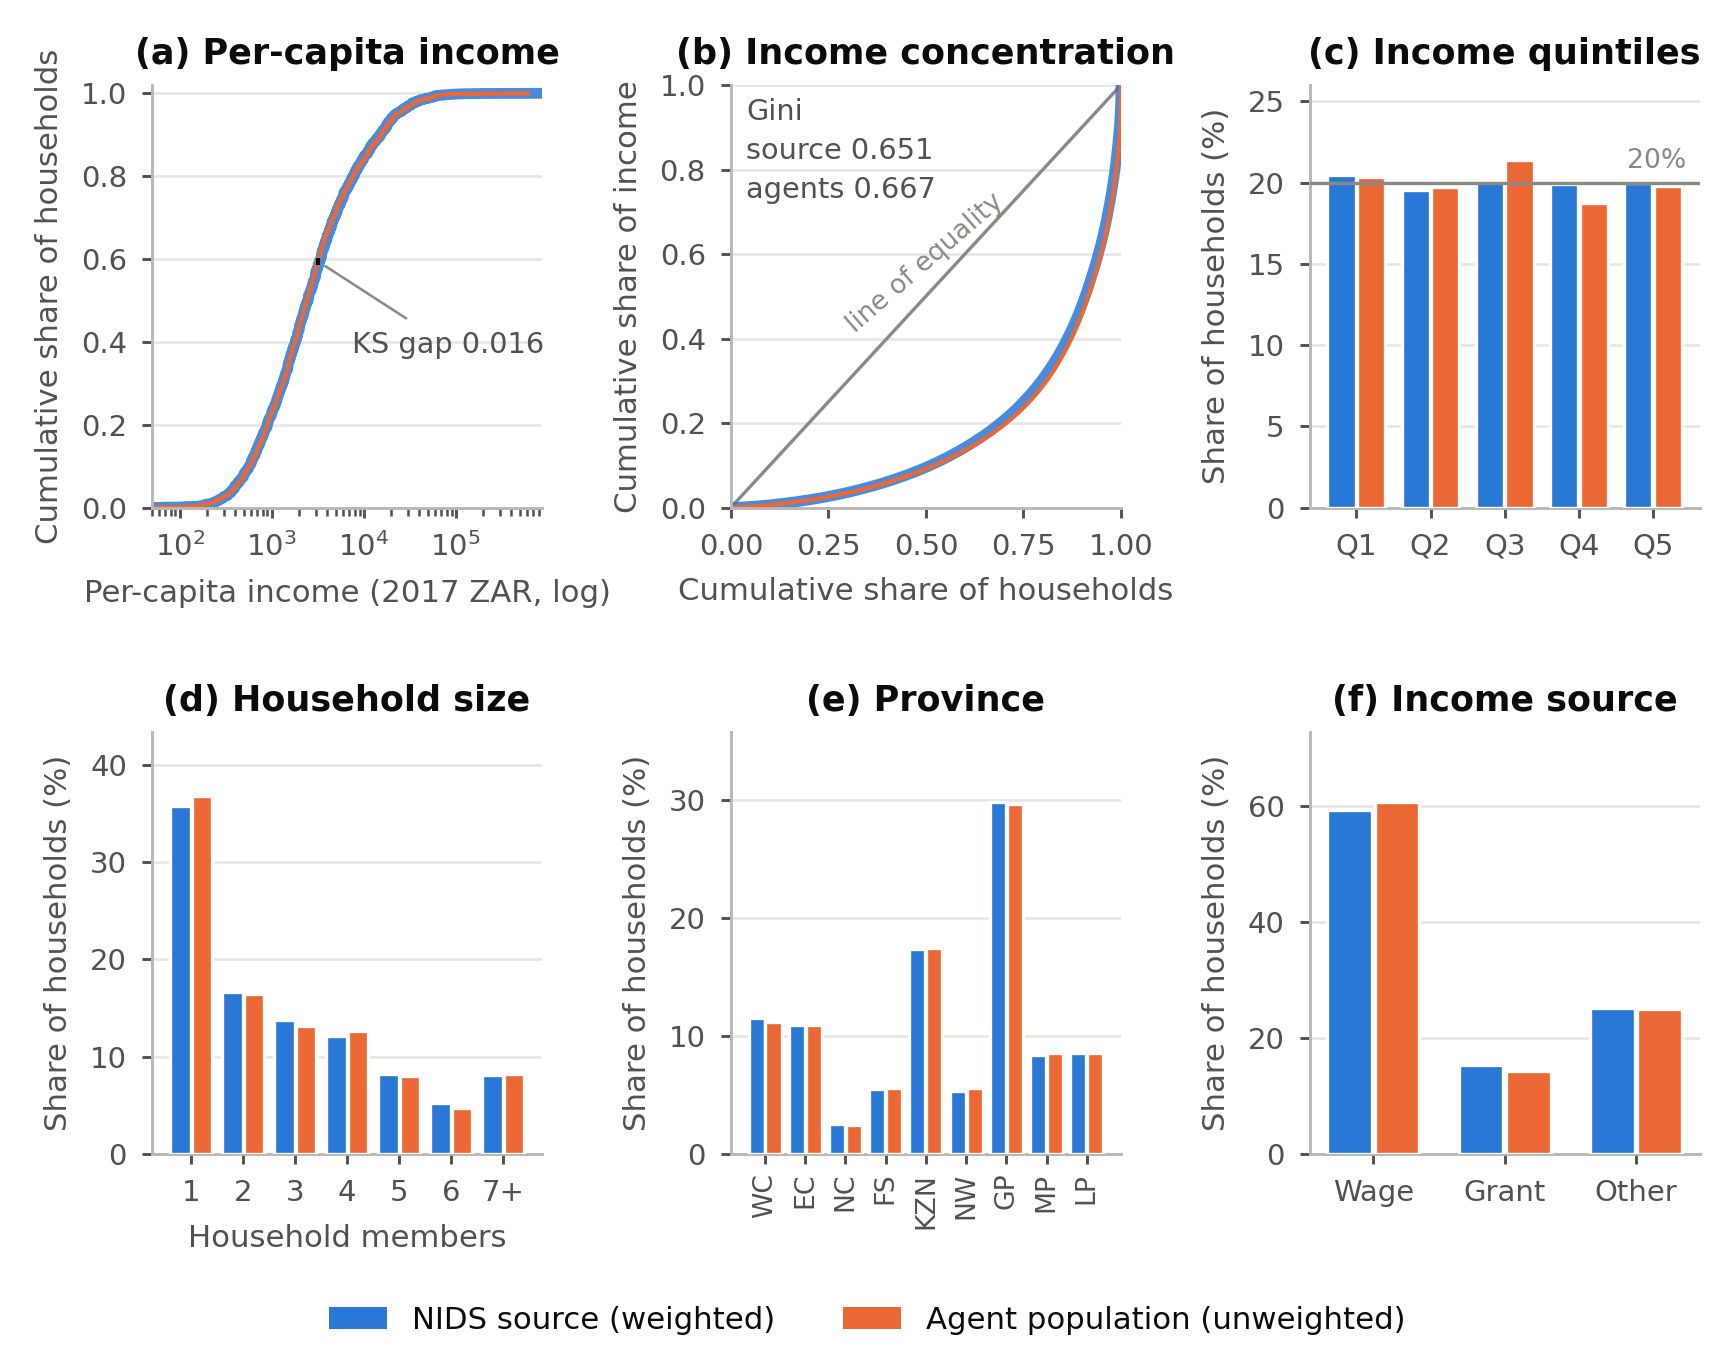
\includegraphics[width=\textwidth]{figures/fig_population_fidelity.pdf}
\caption{Distributional fidelity of the agent population}
\label{fig:pop-fidelity}
\tabnote{Each panel compares the unweighted 5{,}000-agent resample, drawn with replacement in proportion to \ac{NIDS} survey weight (seed 20260818), against the weighted 10{,}841-household source it is drawn from. Panels (a) and (b) cover the per-capita income distribution and its concentration; panels (c) to (f) cover income quintile, household size, province and primary income source, the categorical attributes that gate behaviour and define the reference groups in the simulation. The Kolmogorov--Smirnov distance in (a) is 0.016, the largest categorical deviation is 1.4 percentage points, and the Gini rises from 0.651 to 0.667.}
\end{figure}

\subsection{Validation of the Synthetic Population}
\label{sec:data-validation}

Table~\ref{tab:validation} reports eighteen checks on the constructed population in five groups, and the headline number is not eighteen.
Fourteen are construction checks that test whether the pipeline did what it was specified to do: internal consistency with \ac{NIDS} (Group A), agreement with the \ac{FinScope} marginals that the match reproduces by construction (Group B), and fidelity of the resample to its weighted source (Group E).
All fourteen pass, and none is evidence about the population beyond the two surveys it was built from.
One (Group D, first row) bounds how often the affordability guard binds.
Three are external, comparing the constructed population with a source no construction step used: the per-capita income Gini against the World Bank estimate and aggregate debt against the \ac{CCMR} gross debtor book (Group C), and the servicing share of outlay against \ac{FinScope}'s self-reported budget shares (Group D).
Two of the three pass; the servicing level exceeds its band, for the reason given in Section~\ref{sec:servicing}.

\begin{table}[H]
\centering
\caption{Data-layer validation scorecard}
\label{tab:validation}
\tabnote{Eighteen checks on the constructed population, grouped by what they test. Groups A (consistency with \ac{NIDS}), B (agreement with the \ac{FinScope} marginals the match reproduces by construction) and E (fidelity of the unweighted 5{,}000-agent resample to the weighted source) are construction checks: they verify the pipeline, not the population. Group C compares against sources that no construction step used. Group D bounds the debt-service construction: the first row is the share of debtors for whom the Regulation 23A cap binds, the second the servicing share of monthly outlay among households holding a modelled product, against \ac{FinScope}'s self-reported range. Tolerances with a source: the household-size band is the 2016 Community Survey \cite{statssa_cs_2016}, the Gini interval is bounded below by the World Bank consumption-based estimate \cite{worldbank_gini_zaf}, and the Group D range is \ac{FinScope}'s \cite{finscope2019}; the remainder are the author's. Values are survey-weighted except in Group E, which compares the unweighted agents with the weighted source.}
\begin{tabular}{L{4.9cm}L{3.6cm}rrc}
\toprule
\textbf{Check} & \textbf{Metric} & \textbf{Value} & \textbf{Tolerance} & \\
\midrule
A. Quintile shares $\approx 20\%$ & max $|$share $-0.20|$ & 0.004 & $\pm$2pp & \checkmark \\
A. Mean household size & weighted mean & 3.03 & 3.3 $\pm$0.5 \cite{statssa_cs_2016} & \checkmark \\
A. No impossible values & negative values & 0 & exact & \checkmark \\
\addlinespace
B. Banked (national) & vs FinScope & 0.4pp & $\pm$3pp & \checkmark \\
B. Store card & vs FinScope & 1.8pp & $\pm$3pp & \checkmark \\
B. Revolving credit & vs FinScope & 0.5pp & $\pm$3pp & \checkmark \\
B. Hire purchase & vs FinScope & 0.5pp & $\pm$3pp & \checkmark \\
B. Short-term loan & vs FinScope & 0.6pp & $\pm$3pp & \checkmark \\
B. Personal loan & vs FinScope & 0.2pp & $\pm$3pp & \checkmark \\
B. By-quintile flags & max over q$\times$flag & 2.3pp & $\pm$5pp & \checkmark \\
\addlinespace
C. Per-capita income Gini & weighted Gini & 0.651 & in (0.63, 0.70) & \checkmark \\
C. Aggregate debt vs \ac{CCMR} & stock $/$ in-scope book & 0.49 & in (0.30, 0.80) & \checkmark \\
\addlinespace
D. Servicing plausible pre-guard & debtors the guard binds & 3.8\% & $\leq$10\% & \checkmark \\
D. Debt service vs \ac{FinScope} & monthly outlay, debtors & 12.8\% & in (6.1, 9.8)\% & $\times$ \\
\addlinespace
E. Resample quintile shares & max $|$unwtd $-$ wtd$|$ & 1.3pp & $\pm$2pp & \checkmark \\
E. Resample flag rates & max $|$unwtd $-$ wtd$|$ & 0.8pp & $\pm$3pp & \checkmark \\
E. Resample income ECDF & KS max gap & 0.016 & $\leq$0.05 & \checkmark \\
E. Resample Gini & $|$agents $-$ source$|$ & 0.015 & $\leq$0.02 & \checkmark \\
\bottomrule
\end{tabular}
\end{table}

The two external checks that pass are informative because nothing in the construction targeted them.
The per-capita income Gini of 0.651 falls within the 0.630--0.700 interval bounded below by the World Bank's consumption-based estimate \cite{worldbank_gini_zaf}, income-based measures in South Africa exceeding consumption-based ones.
Total synthetic population debt (ZAR 191.4 billion) is 49\% of the corresponding \ac{CCMR} gross debtor book (ZAR 392.0 billion) \cite{ncr_ccmr_2017}, a ratio consistent with the self-reporting undercount usual in micro-surveys relative to administrative registers; it also supports the zero-fill choice of Section~\ref{sec:backbone}, since imputing missing debt at holder means would give aggregate debt equal to 111\% of the entire administrative book.

Two structural deviations remain. Mean household size (3.03) passes tolerance but sits below the 3.3 estimate from the 2016 Community Survey \cite{statssa_cs_2016}; because weighted population totals match national benchmarks, this generates roughly 10\% more household units (18.67 million against 16.9 million).
And the synthesised population exhibits baseline financial vulnerability before any simulation runs: at initialisation, 3.9\% of households cannot cover committed expenditure from income, 5.2\% cannot cover committed outlays plus scheduled debt service, and 44.3\% hold zero liquid savings.
Under the default rules of Section~\ref{sec:submodels}, these households register distress at $t=0$ independent of experimental shocks or \ac{BNPL} availability.

\subsection{Agent Attribute Mapping}
\label{sec:agent-mapping}

Table~\ref{tab:agent-mapping} summarises the state variables initialised for each agent. Variables map directly to microdata observations, structural imputations, or derived accounting rules; unused survey fields are excluded.

\begin{table}[H]
\centering
\caption{Data-to-agent mapping}
\label{tab:agent-mapping}
\tabnote{The state variables initialised for each agent, their meaning, and their source. Monetary fields are 2017 Rands. Fields marked \emph{tick} are monthly survey flows scaled by $12/26$ to the 14-day tick; stocks (savings, debt) are not scaled. Construction detail for every derived field is in Appendix~\ref{app:variables}; the imputed flags are described in Section~\ref{sec:match} and Appendix~\ref{app:matching}. Two dimensions are not observed in the microdata: every agent starts with a zero \ac{BNPL} balance, which is the injection design, and the repayment archetype of Section~\ref{sec:submodels} is assigned at random at initialisation.}
\begin{tabular}{L{4.8cm}L{4.4cm}L{4.2cm}}
\toprule
\textbf{Agent field} & \textbf{Description} & \textbf{Source} \\
\midrule
\texttt{income\_monthly} & Total monthly liquidity inflows & NIDS \\
\texttt{income\_wage\_tick} & Wage component; the base a shock removes & NIDS \\
\texttt{n\_earners} & Employed members on the roster & NIDS individual file \\
\texttt{income\_source} & Dominant component: wage, grant, other & NIDS, derived \\
\texttt{committed\_tick} & Incompressible food and rent costs & NIDS, derived \\
\texttt{discretionary\_tick} & Non-food expenditure & NIDS, derived \\
\texttt{liquid\_savings} & Proxy for immediate cash buffer & NIDS, winsorised \\
\texttt{d\_trad} & Outstanding traditional debt balance & NIDS \\
\texttt{apr\_annual}, \texttt{term\_months} & Rate and horizon pricing that balance & Product mix (Section~\ref{sec:servicing}) \\
\texttt{scheduled\_service\_tick} & Monthly debt servicing obligation & Constructed (Section~\ref{sec:servicing}) \\
\texttt{nca\_capacity\_monthly} & Regulation 23A affordable residual & Statutory (Section~\ref{sec:servicing}) \\
\texttt{banked} & Eligibility gate for \ac{BNPL} & FinScope, imputed \\
\texttt{income\_quintile} & Relative wealth bracket; donor match key & NIDS, weighted \\
\texttt{province} & Geographic tag; donor match key & NIDS \\
\texttt{reference\_group} & Network topology for peer adoption observation & Derived (quintile $\times$ province) \\
\texttt{household\_size} & Total household members & NIDS \\
\bottomrule
\end{tabular}
\end{table}
